\documentclass[a4paper,10pt]{article}
\usepackage[utf8x]{inputenc}
\usepackage{algorithm}
\usepackage{algorithmic}
\usepackage[T1]{fontenc}
\usepackage[centertags]{amsmath}
\usepackage{amssymb,amsmath}
\usepackage[margin=1.0in]{geometry}
\usepackage{url}
\usepackage{bera}
\usepackage{draftcopy}
\usepackage{graphicx}
\usepackage{epsfig}
%opening
\title{Computation of hopping amplitudes in a 2D Honeycomb optical lattice}
\author{Analabha Roy}

\begin{document}

\maketitle

\section{The Hexagonal Lattice}
Our 2D potential of interest is given by~\cite{laetitia}
\begin{equation}
\label{eq:pot}
v({\bf r}) = v_{\bar{x}}\sin^2{x}  + v_x\cos^2{x} +  v_y\cos^2y + 
  2 \sqrt{v_x v_y}\cos{x}\cos{y},
\end{equation}
where all energy parameters have been scaled with the recoil energy $E_R\equiv \hbar^2 k^2/2m$ and lengths scaled with the 
laser wavelength $\lambda=2\pi/k$. The derivatives of the potential are
\begin{eqnarray}
\partial_x v(x,y) &=& -2\sin{x}\left[\left(v_x-v_{\bar{x}} \right) \cos{x} + 2\sqrt{v_xv_y}\cos{y}\right], \nonumber \\
\partial_y v(x,y) &=& -2\sin{y}\left[ v_y \cos{y} + 2\sqrt{v_xv_y}\cos{x}\right].
\end{eqnarray}
The extrema lie at the points where both derivatives vanish i.e., when
\begin{eqnarray}
\label{eq:extrema}
\left(x,y \right) &=& \left(n\pi,m\pi \right), \nonumber \\
\left(x,y \right) &=& \left(\left\{2n+1\right\}\pi/2,\left\{2m+1\right\}\pi/2 \right), \nonumber \\
\left(x,y \right) &=& \left(n\pi,2m\pi\pm\cos^{-1}\left\{2(-1)^{n+1}\sqrt{\frac{v_x}{v_y}}\right\} \right),\nonumber \\
 \left(x,y \right) &=& \left(2n\pi \pm \cos^{-1}\left\{2(-1)^{m+1}\frac{\sqrt{v_xv_y}}{v_x-v_{\bar{x}}} \right\},m\pi \right).
\end{eqnarray}
Here, the rarely occurring solution when $(v_x-v_{\bar{x}})v_y-2v_xv_y=0$ has been ignored. The final roots of eq~\ref{eq:extrema} produce minima. The first two produce saddles and the third produce maxima. This can be shown by computing the Hessian, or inferred from fig~\ref{fig:potn}. We now define a size parameter for this lattice by
\begin{equation}
\label{eq:d}
\delta\equiv\cos^{-1}\left\{\frac{2\sqrt{v_xv_y}}{v_x-v_{\bar{x}}}\right\}. 
\end{equation}
The final roots of eq~\ref{eq:extrema} can be broken down to
\begin{eqnarray}
\label{eq:minima}
 \left[x,y \right] &=& \left[2n\pi \pm \delta,\left(2m+1\right)\pi \right], \nonumber \\
\left[x,y \right] &=& \left[\left(2n+1\right)\pi \pm \delta,2m\pi \right].
\end{eqnarray}
\begin{figure}[h!bt]
\ 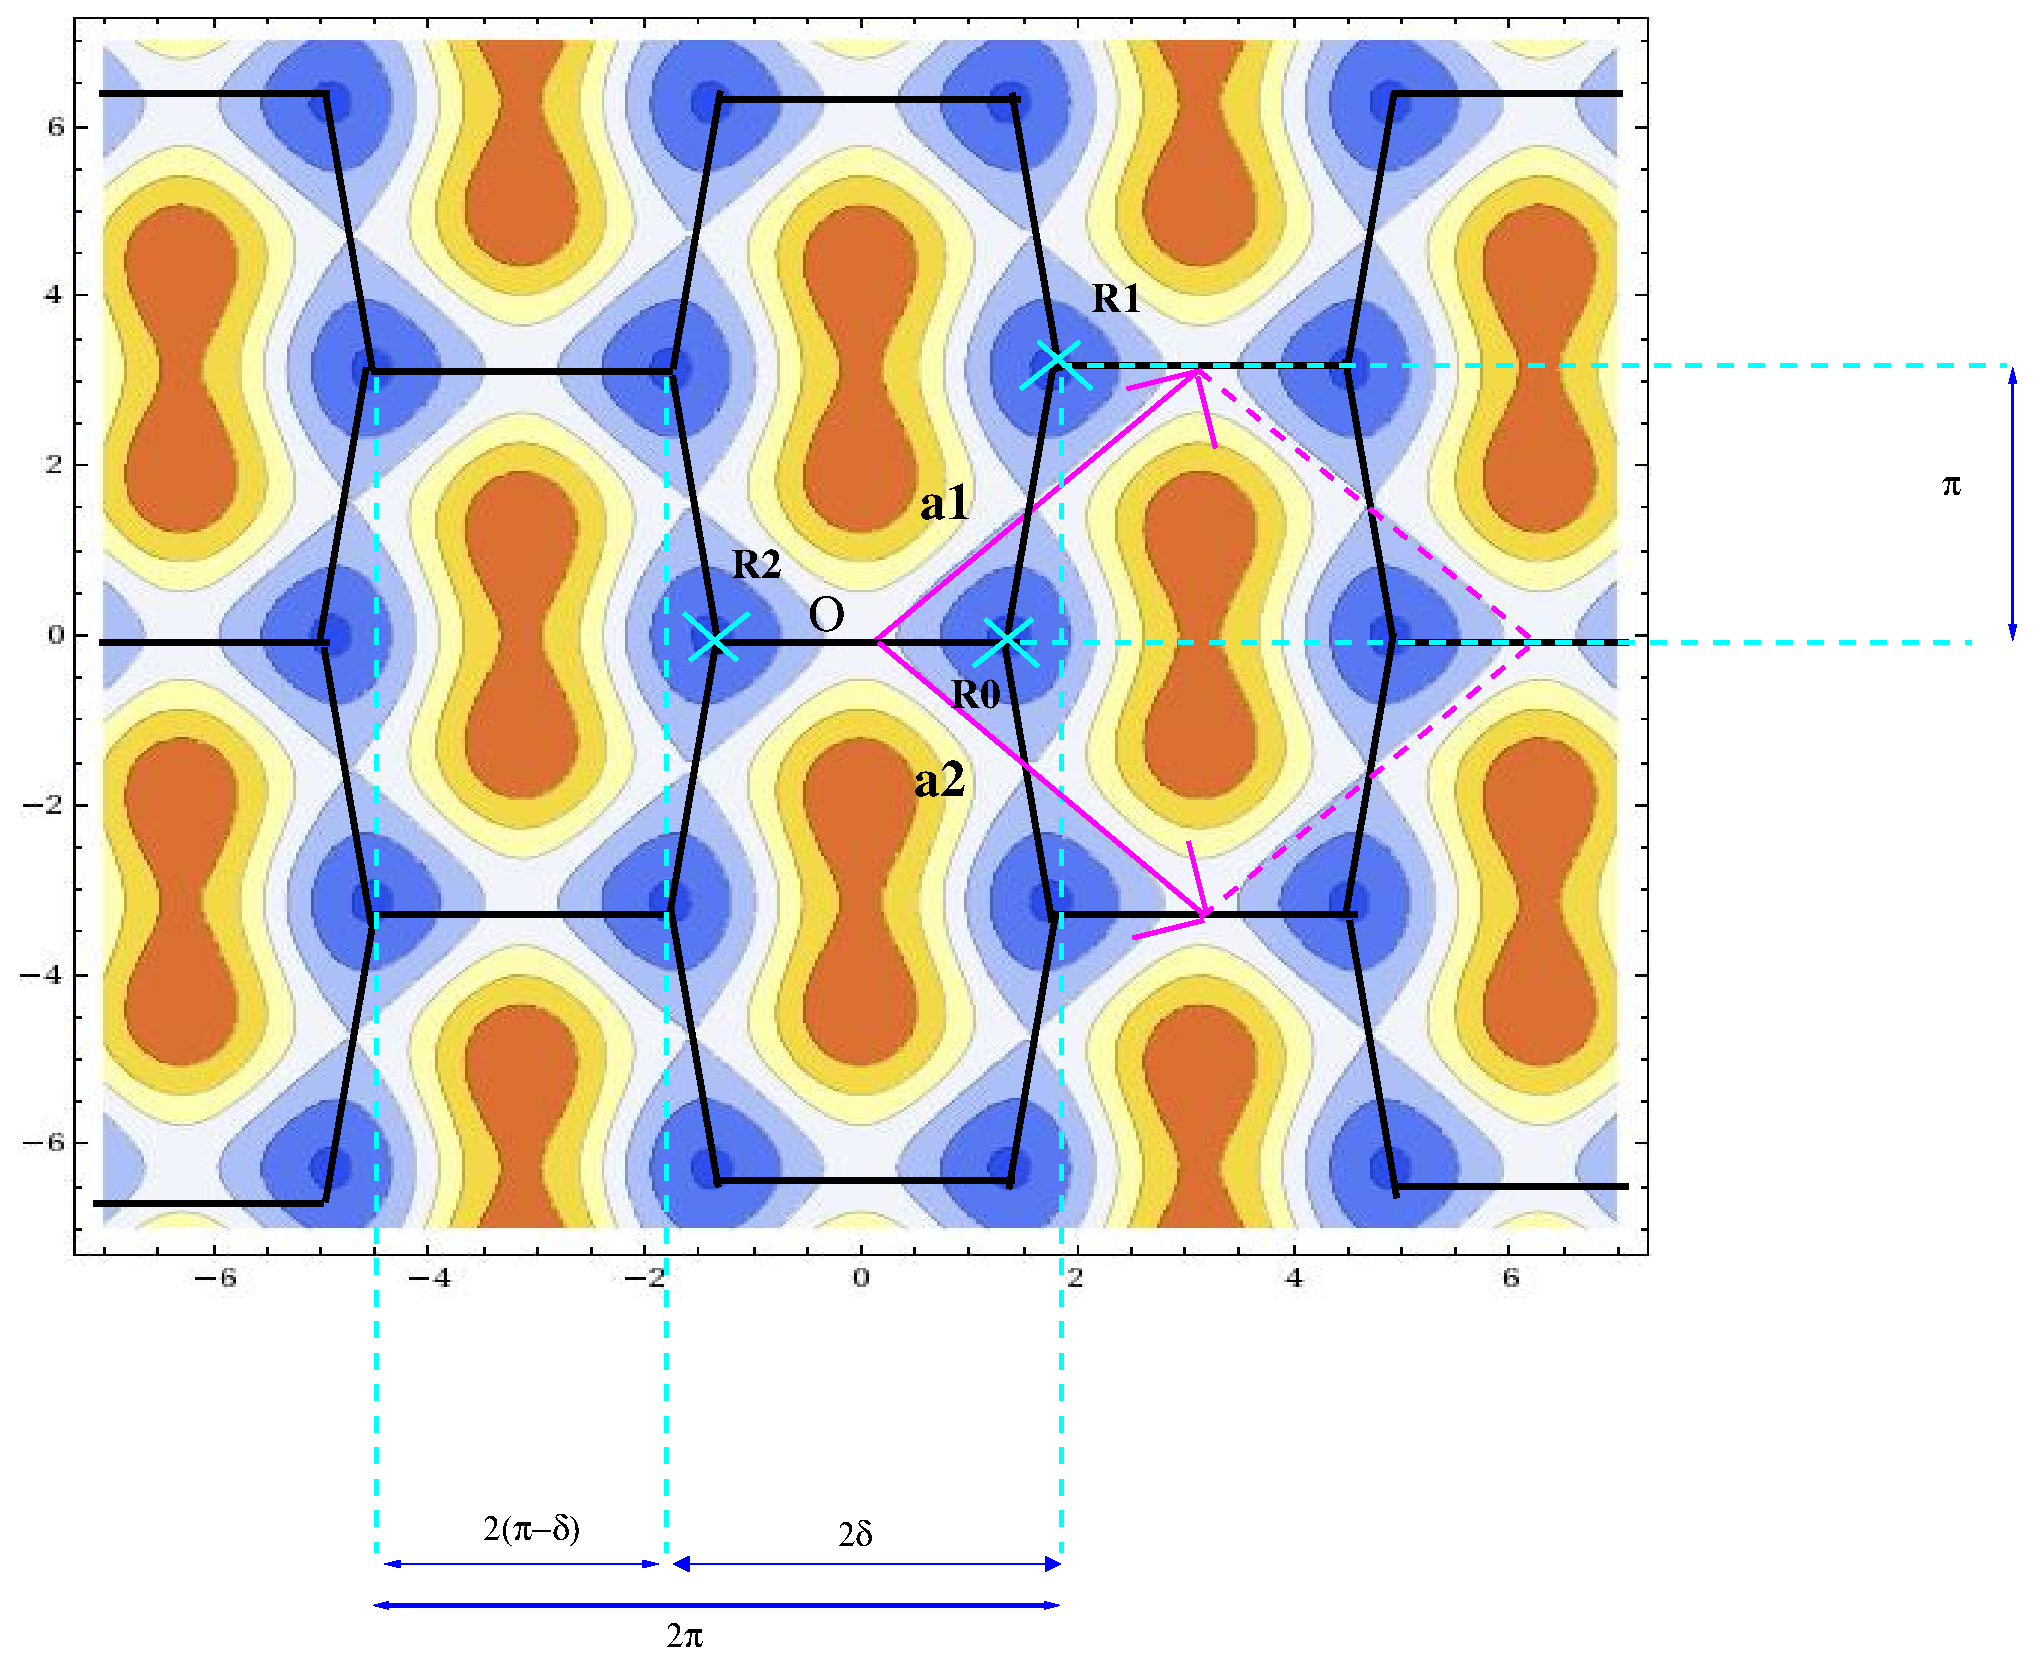
\epsfig{file=potn.eps,height=5.0in,width=5.3in}
\caption{This figure shows a plot of $v(x,y)$ for $v_x=0.25$, $v_{\bar{x}}=4.0$,$v_y=2.0$ in units of $E_R$. The hexagonal structure of the potential minima is indicated via the black solid lines in overlay. The unit cell of the trigonal Bravais lattice with $2$-atom basis is shown in  magenta. The two vectors that generate this lattice are given by the magenta vectors ${\bf a}_1$ and ${\bf a}_2$. Also, $\delta$ is given by eq~\ref{eq:d}. The three sites which are to be used for calculating hopping amplitudes are shown as cyan crosses labeled ${\bf R}_i$.}
\label{fig:potn}
\end{figure}
We now make the following observations based on fig~\ref{fig:potn} and equations~\ref{eq:d},~\ref{eq:minima}:
\begin{enumerate}
 \item 
At $\delta=\pi/2$, the lattice becomes a series of 1d chains. This happens when $v_{\bar{x}}\gg v_x$, in accordance with~\cite{laetitia}.
\item
As we increase $\delta$ from $\pi/2$, the structure becomes hexagonal. A sample is plotted in fig~\ref{fig:potn}. Here, the base width of the hexagonal unit cell is $2\delta$, the vertical height is $2\pi$, and the horizontal length is $2(\pi-\delta)$. Thus, the size parameter uniquely specifies the dimensions of the honeycomb lattice, with the horizontal edge decreasing in length while the base width increases, when the horizontal edge becomes smaller than half the base width, the lattice becomes one of dimers. Therefore, the boundary between hexagonal and dimer regimes in the parameter space is given by the equation $2(\pi-\delta)=\delta$, solving to $\delta=2\pi/3$. From eq~\ref{eq:d}, we get
\begin{equation}
 \label{eq:hcdbound}
{v_{\bar{x}}-v_{x}} = {4\sqrt{v_xv_y}}.
\end{equation}
\item
As $\delta\rightarrow 2\pi$ from $2\pi/3$, the lattice assumes a triangular structure, and tends to a dimer structure. This becomes dimer for $\delta\gtrsim2\pi$. Thus, the boundary between triangular regime and dimer regime in the parameter space is given by the curve
\begin{equation}
 \label{eq:tdbound}
{v_{\bar{x}}-v_{x}} = {2\sqrt{v_xv_y}}.
\end{equation}
\end{enumerate}
These regimes are indicated in fig~\ref{fig:params}. We conclude from eq~\ref{eq:hcdbound} and fig~\ref{fig:params} that the hexagonal regime is given by the region containing the points for which
\begin{equation}
 \label{eq:hcregime}
v_{\bar{x}} - \left(v_x + 4 \sqrt{v_xv_y}\right) \geq 0.
\end{equation}
However, if $v_{\bar{x}}\gg v_x$, these hexagons will become 1d chains. 

In the hexagonal/honeycomb regime, the unit cell is generated by the basis vectors ${\bf a}_1$ and ${\bf a}_2$ as shown by magenta arrows in fig~\ref{fig:potn}. Each unit cell contains two sites, and integer multiples of these vectors build the entire lattice, with the atoms in the cell forming a sublattice (two total) with the corresponding atoms in all the unit cells. The basis vectors are given by
\begin{eqnarray}
\label{eq:basis}
{\bf a}_1 &=& 2\left(\pi-\delta\right)\hat{x} + \pi \hat{y},\nonumber \\
{\bf a}_2 &=& 2\left(\pi-\delta\right)\hat{x}-\pi \hat{y}.
\end{eqnarray}
\begin{figure}[h!bt]
\ 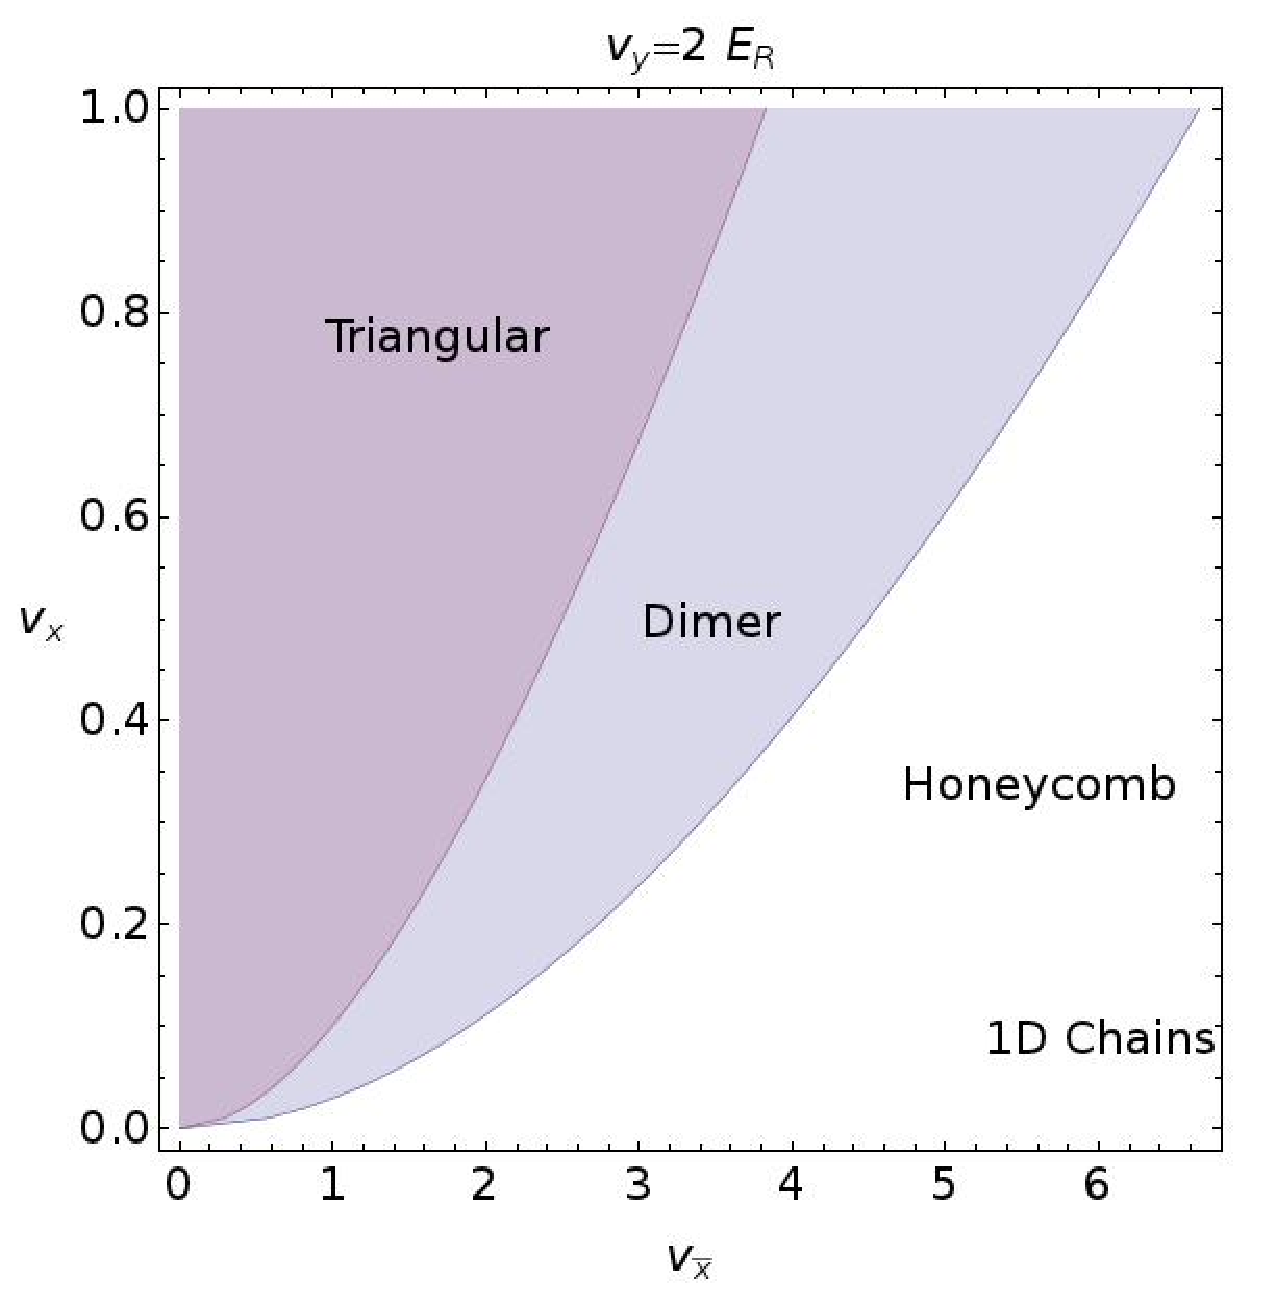
\epsfig{file=v1v2_data.eps,height=4.5in,width=4.5in}
\caption{This figure shows the accessible lattice geometries as a function of the lattice depths $v_{\bar{x}}$ and $v_x$ in units of the recoil energy $E_R$. The plots are for $v_y=2.0$. The region where the system realizes honeycomb packing is indicated.}
\label{fig:params}
\end{figure}
The reciprocal lattice will be generated by the basis vectors ${\bf b}_1$ and ${\bf b}_2$ that satisfy the condition ${\bf b}_i \cdot {\bf a}_j = 2\pi \delta_{ij}$. After some algebra, these are obtained to be
\begin{eqnarray}
\label{eq:basis:recip}
{\bf b}_1 &=& \alpha \hat{x} + \hat{y},\nonumber \\
{\bf b}_2 &=& \alpha \hat{x}- \hat{y},\nonumber \\
\alpha &\equiv& \left[2\left(1-\frac{\delta}{\pi}\right)\right]^{-1}.
\end{eqnarray}
The quantity $\alpha$ is now the size parameter of the reciprocal lattice. As the real space lattice gets bigger (increasing $\delta$), the reciprocal lattice gets smaller (decreasing $\alpha$). The reciprocal lattice is constructed in fig~\ref{fig:bzone}. The vectors ${\bf b}_i$ are indicated in magenta, and the corresponding first Brillouin zone (FBZ) is indicated in blue. The FBZ is formed by the perpendicular bisectors of ${\bf b}_{1,2}$ and their mirror images. The lines are labeled $L_{1,2}$ and their mirror images $L'_{1,2}$. The equations of these lines can be obtained after some algebra.Thus the criteria for a crystal momentum ${\bf k}$ being inside the FBZ is given by 
\begin{equation} 
\label{eq:bzone}
\begin{array}{rcl} 
L_1  :& \alpha k_y+k_x-\alpha   &\leq0 , \\
L_2  :&  \alpha k_y-k_x-\alpha  &\leq0 , \\
L'_1  :& \alpha k_y+k_x+\alpha  &\geq0 , \\
L'_2  :& \alpha k_y-k_x+\alpha  &\geq0 .
\end{array}
\end{equation}
\section{The Hopping Amplitudes}
Based on the previous sections, the algorithm for obtaining the hopping amplitudes can be written down. The full exact Hamiltonian is reformulated for crystal momentum ${\bf k}$ as a matrix in real space. This yields
\pagebreak
\begin{figure}[h!bt]
\ 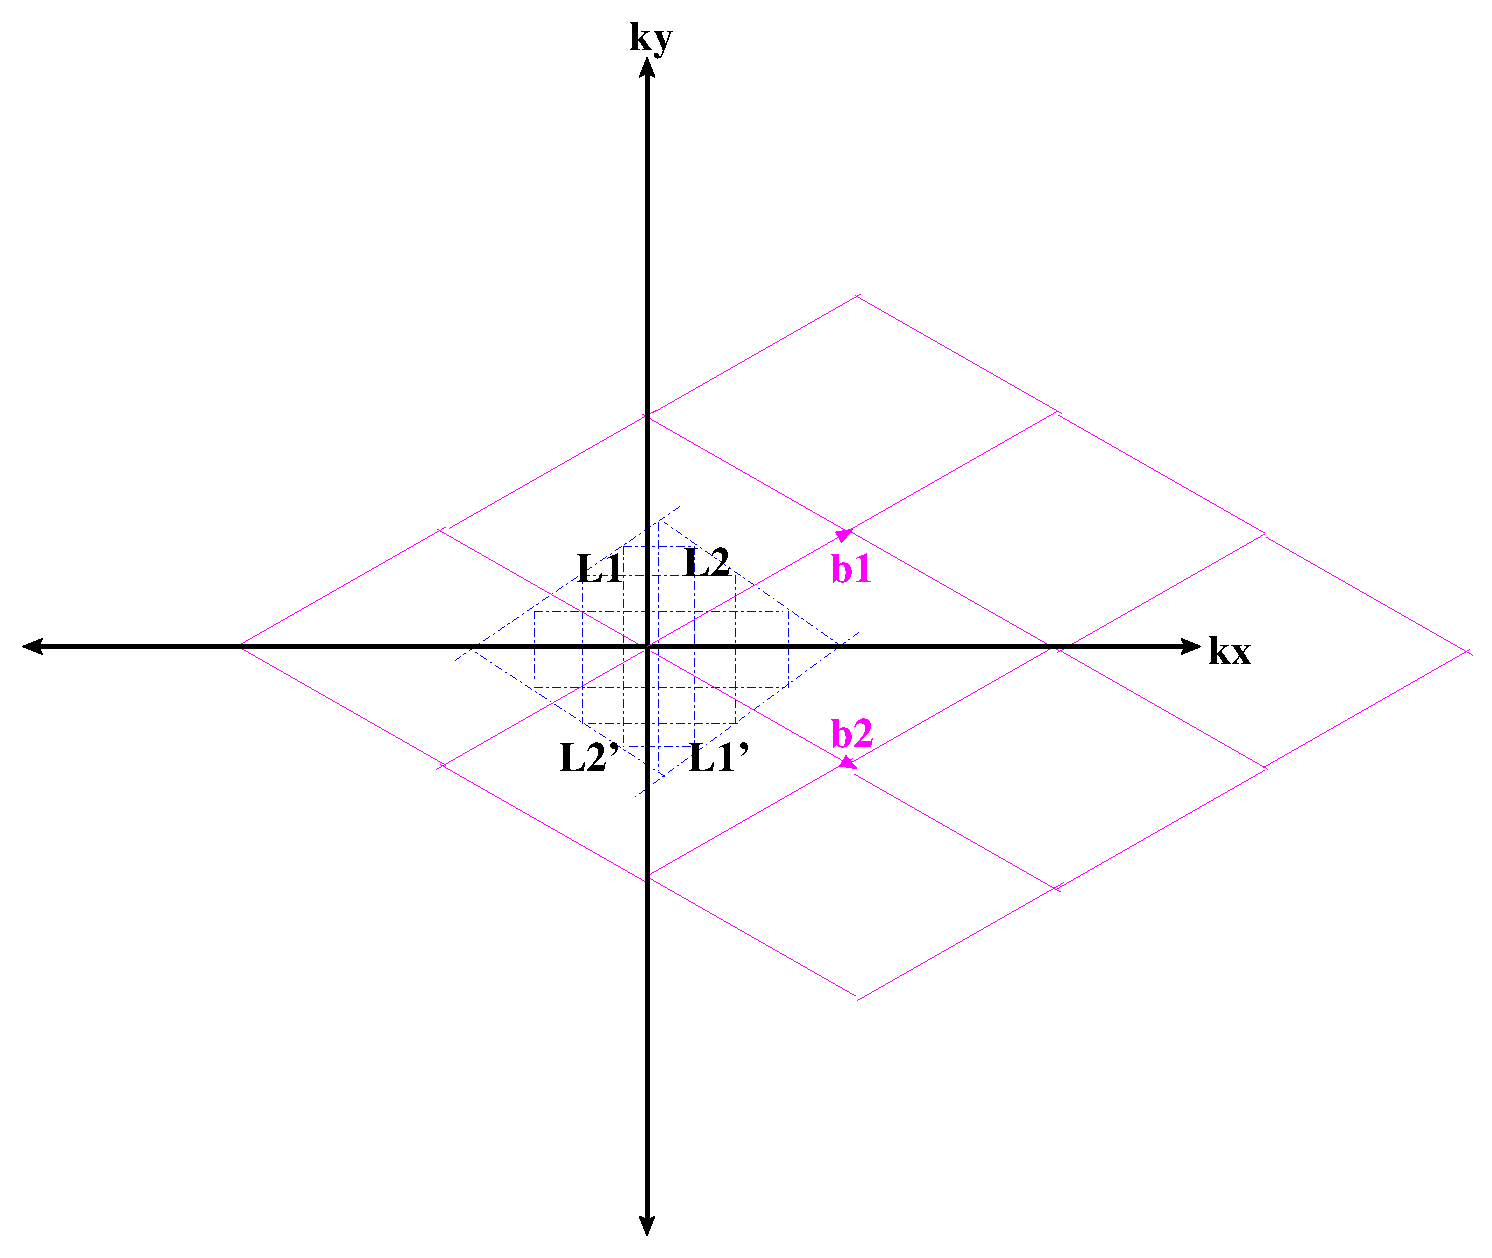
\epsfig{file=bzone.eps,height=4.5in,width=4.5in}
\caption{The reciprocal lattice of the trigonal Bravais lattice in fig~\ref{fig:potn}. The basis vectors are ${\bf b}_{1,2}$. The lines $L_i$ and $L'_i$ bound the FBZ of the lattice as shown in blue.}
\label{fig:bzone}
\end{figure}
\begin{equation}
\mathcal{H}_{\bf k} = \frac{1}{2}\left(-i\vec{\nabla} + {\bf k} \right)^2 + v({\bf r}).
\end{equation}
The eigenvalue equation provides the energy band structure $\epsilon^{n}_{\bf k}$ and the Bloch eigenstates $|{n}, {\bf k},{\bf r}\rangle$ viz.
\begin{equation}
\mathcal{H}_{\bf k} |{n}, {\bf k},{\bf r}\rangle = \epsilon^{n}_{\bf k} |n,{\bf k}, {\bf r}\rangle,
\end{equation}
where $n$ is the band index. We rasterize this Hamiltonian in real space as follows. First, we rasterize real space in a grid of size $N$ running from a cutoff $[-C,C]$ in steps of $d$. This way the continuous vector $|{\bf r}\rangle$
(where the $n,{\bf k}$ have been dropped) is mapped to a discreet array as 
\begin{equation}
|{\bf r}\rangle \rightarrow |{\bf r}_{\alpha}\left(x_i,y_j\right)\rangle.
\end{equation}
Here, the Roman indices $i,j$ run in the range $[0,N-1]$, and the Greek index $\alpha = i + N j$. Thus, the Greek indices run in the range $[0,N^2-1]$. The gradients and Laplacians in the Hamiltonian are mapped as
\begin{equation}
\left(-i\vec{\nabla}+{\bf k} \right) |{\bf r}\rangle \rightarrow \left[k_x |{\bf r}_{\alpha}\rangle-i\frac{|{\bf r}_{\alpha+1}\rangle-|{\bf r}_{\alpha-1}\rangle}{2d} \right] \hat{x} + \left[k_y |{\bf r}_{\alpha}\rangle -i\frac{|{\bf r}_{\alpha+N}\rangle-|{\bf r}_{\alpha-N}\rangle}{2d} \right]\hat{y}, \nonumber \\
\end{equation}
Taking 2 sets of indices $\beta = p+Nq$ and $\beta' = p'+Nq'$ that run in the same range as $\alpha$, the discretized Hamiltonian is obtained from the equations above and using the orthonormality of the $|{\bf r}\rangle$s. The result is
\begin{multline}
\label{eq:hamilt}
H_{\beta \beta'} = \left(\frac{k^2}{2}-v_\beta\right)\delta_{\beta\beta'} - i\frac{k_x}{2d}\left(\delta_{\beta,\beta'+1}+\delta_{\beta,\beta'-1}\right)-i\frac{k_y}{2d}\left(\delta_{\beta,\beta'+N}-\delta_{\beta,\beta'-N}\right) \\
-\frac{1}{8d^2}\left(\delta_{\beta,\beta'+2}+\delta_{\beta,\beta'-2}+\delta_{\beta,\beta'+2N}+\delta_{\beta,\beta'-2N} - 4\delta_{\beta\beta'} \right).
\end{multline}
In the above equation, the expression $v_\beta = v(x_p,y_q)$ taken from eqn~\ref{eq:pot}. The above Hamiltonian can be numerically diagonalized for a suitable choice of $C,N$ for all crystal momenta in FBZ given by eq~\ref{eq:bzone}, which is also discretized with a cutoff $M$. Thus, the problem size is determined by the set $[C,N,M]$. The two eigenvalues on either side of $0$,  $\epsilon^\pm_{\bf k}$ and their corresponding Bloch eigenfunctions $|\pm, {\bf k},{\bf r}\rangle$ are what we seek to obtain. The computations are detailed in algorithm~\ref{alg:main} below. 

Now, the Wannier functions localized at a particular lattice site ${\bf R}$ in the lattice $L_h$ are given by~\cite{rossler}
\begin{equation}
|n,{\bf R},{\bf r}\rangle  = \frac{\mathcal V}{4\pi^2}\int_{FBZ}{\mathrm d}^2k \times e^{-i{\bf k}\cdot\left({\bf R}-{\bf r} \right)}|n,{\bf k}, {\bf r}\rangle.
\end{equation}
Here, ${\mathcal V}$ is the volume of the real space primitive cell that generates $L_h$. In our case, this can be seen from fig~\ref{fig:potn} to be $2\pi^2$, independent of $\delta$. The hopping amplitude between the origin ${\bf R}_0$ and another lattice site ${\bf R}_i$ is~\cite{rossler}
\begin{equation}
\tau_i = \frac{1}{2M^2}\sum^{FBZ}_{\bf k}\left(\epsilon^+_{\bf k} - \epsilon^-_{\bf k} \right) \times e^{i{\bf k}\cdot\left({\bf R}_0-{\bf R}_i \right)},
\end{equation}
where $M$ is the momentum space grid size. If we choose half the FBZ, ie the top half (call it HFBZ), then for every ${\bf k}$ in HFBZ there is a $-{\bf k}$ in the lower half, and the equation above can be simplified to
\begin{equation}
 \label{eq:tau}
\tau_i = \frac{1}{M^2}\sum^{HFBZ}_{\bf k}\left(\epsilon^-_{\bf k} - \epsilon^+_{\bf k} \right) \times \cos\left[{{\bf k}\cdot\left({\bf R}_0-{\bf R}_i \right)}\right].
\end{equation}
The two unique hopping amplitudes lie between the vectors ${\bf R}_0$ and ${\bf R}_{1,2}$ as indicated in fig~\ref{fig:potn}.
\begin{eqnarray}
\label{eq:hoppingvecs}
{\bf R}_0 &=& \left(\pi-\delta\right)\hat{x}  , \nonumber \\
{\bf R}_1 &=& \left(2\delta-\pi\right)\hat{x} + \pi\hat{y} , \nonumber \\
{\bf R}_2 &=& \left(\delta-\pi\right)\hat{x} .
\end{eqnarray}
Once $\epsilon_\pm$ are known numerically, $\tau_{1,2}$ can be computed from the above equation for each point in the parameter space.
\begin{algorithm}                      % enter the algorithm environment
\caption{Calculate hopping amplitudes $\tau_1$ and $\tau_2$ and dump out full band structure}          % give the algorithm a caption
\label{alg:main}                           % and a label for \ref{} commands later in the document
\begin{algorithmic}                    % enter the algorithmic environment
\REQUIRE $v_x$, $v_{\bar{x}}$ $v_y$, the three cutoffs $[C,N,M]$, and a default crystal momentum bound $K$.
\ENSURE That the condition for hexagonality, eq~\ref{eq:hcregime}, is met.
\STATE Evaluate mesh unit from mesh size input.
\STATE Create object krange for storing range of momenta.
\STATE Create object kdata for storing momentum and energy data. 
\STATE Evaluate $\delta$ from eqn~\ref{eq:d}.
\STATE Evaluate lattice sites ${\bf R}_{1,2,3}$ from eqns~\ref{eq:hoppingvecs}.
\STATE Evaluate $\alpha$ and ${\bf b}_i$ from eqns~\ref{eq:basis:recip}.
\STATE
\STATE \COMMENT{Now, Build a range of momenta ${\bf k}$ that encompasses the FBZ.} 
\STATE Call subroutine~\ref{alg:fbz}.
\STATE 
\STATE Initiate ${\bf k}$ from first value in krange.
\FOR{${\bf k}$ in krange}
\STATE Create hamiltonian object.

\STATE Initiate counter $p=0$.
\WHILE{$p\leq N$}
\STATE Initiate counter $q=0$
\WHILE{$q\leq N$}
\STATE Initiate counter $p'=0$
\WHILE{$p'\leq N$}
\STATE Initiate counter $q'=0$
\WHILE{$q'\leq N$}
\STATE Evaluate $\beta = p + Nq$.
\STATE Evaluate $\beta'  = p' +Nq'$.
\STATE Evaluate Hamiltonian matrix element from eqns~\ref{eq:hamilt}.
\STATE Append this element and the indices $\beta,\beta'$ to the hamiltonian object.
\STATE Increment $q'$.
\ENDWHILE
\STATE Increment $p'$.
\ENDWHILE
\STATE Increment $q$.
\ENDWHILE
\STATE Increment $p$.
\ENDWHILE

\STATE Diagonalize the hamiltonian.
\STATE Obtain the two eigenvalues on either side of $0$,  $e^-_{\bf k},e^+_{\bf k}$.
\PRINT ${\bf k},e_-,e_+$.
\STATE Append ${\bf k},e_-,e_+$ to kdata.
\STATE Clear hamiltonian object.
\ENDFOR
\STATE
\STATE \COMMENT{Calculate the hopping amplitudes $\tau_{1,2}$}.
\STATE $\tau_1=$ call of subroutine~\ref{alg:hopping} with ${\bf R}_0, {\bf R}_1$.
\STATE $\tau_2=$ call of subroutine~\ref{alg:hopping} with ${\bf R}_0, {\bf R}_2$.
\PRINT $\tau_{1,2}$.
\end{algorithmic}
\end{algorithm}
\floatname{algorithm}{Subroutine}
\begin{algorithm}
\caption{Build the First Brillouin Zone of the lattice in fig~\ref{fig:bzone}}
\label{alg:fbz}                           % and a label for \ref{} commands later in the document
\begin{algorithmic}                    % enter the algorithmic environment
\REQUIRE Memory location of object krange,mesh size of crystal momenta,$K$, and $\alpha$.
\FOR{${\bf k}$ in the range $K$}
\IF{${\bf k}$ satisfies eqns~\ref{eq:bzone}}
\STATE append ${\bf k}$ to krange
\ENDIF
\STATE Increment ${\bf k}$ by mesh size.
\ENDFOR
\end{algorithmic}
\end{algorithm}
\begin{algorithm}
\caption{Calculate the hopping amplitudes $\tau_{1,2}$.}
\label{alg:hopping}                           % and a label for \ref{} commands later in the document
\begin{algorithmic}                    % enter the algorithmic environment
\REQUIRE ${\bf R}_{1,2}$ from main, memory location to objects krange, and kdata.
\STATE Initiate ${\bf k}$ as first element of krange.
\STATE Initiate $\tau=0$.
\FOR{${\bf k}$ in krange} 
\STATE Extract the corresponding $e_\pm$ from kdata.
\STATE Update the sum of eqns~\ref{eq:tau} to $\tau$.
\ENDFOR
\STATE Return $\tau$.
\end{algorithmic}
\end{algorithm}
\pagebreak
\begin{table}[h!bt]
\begin{center}
\begin{tabular}{ | l  l  l  l l l|| l | l |}
      \hline
  $v_{\bar{x}}$ 	&$v_x$  &$v_y$ &$C$ &$N$ &$M$	& $\tau_0$    & $\tau_1$ \\  \hline  \hline
  $4.0$			&$0.25$	&$2.0$ &$100$ &$50$ &$50$ &$0.000863248545$ &$0.001317922756$ \\ \hline
     \end{tabular}
\caption{Parameters and results for a single run of the algorithm~\ref{alg:main}. The real space lattice was rasterized in a grid of $N\times N$ elements with $x$ and $y$ ranging from $(-C,-C)$. The FBZ in momentum space (bounded by the lines in eqn~\ref{eq:bzone}) was rasterized in a grid of size $M\times M$. The left columns show the values of the parameters chosen for this run, as well as the potential amplitudes in eqn~\ref{eq:pot}. The right columns show the hopping amplitudes obtained from eqns~\ref{eq:tau} using eqns~\ref{eq:hoppingvecs}. All quantities are expressed in units of the lattice recoil energy $E_R$ with $\hbar=1$.}
\label{tab:params:tau}
\end{center}
\end{table}
\section{Results:}
The algorithms above have been implemented in $C$ with parallelization achieved via the MPI Message Passing Interface. A sample run has been made for the parameters in table~\ref{tab:params:tau}. The calculated hopping amplitudes $\tau_{0,1}$ are also shown there. The entire run took $2400$ seconds using $36$ processors in parallel. The band structure obtained for these parameters is shown in fig~\ref{fig:bands:3d}. Furthermore, fig~\ref{fig:lband:contour} shows contour plots of the lower energy band, with possible candidates for the $K$ and $K'$ points of graphene.
\pagebreak
\begin{figure}[h!bt]
\ 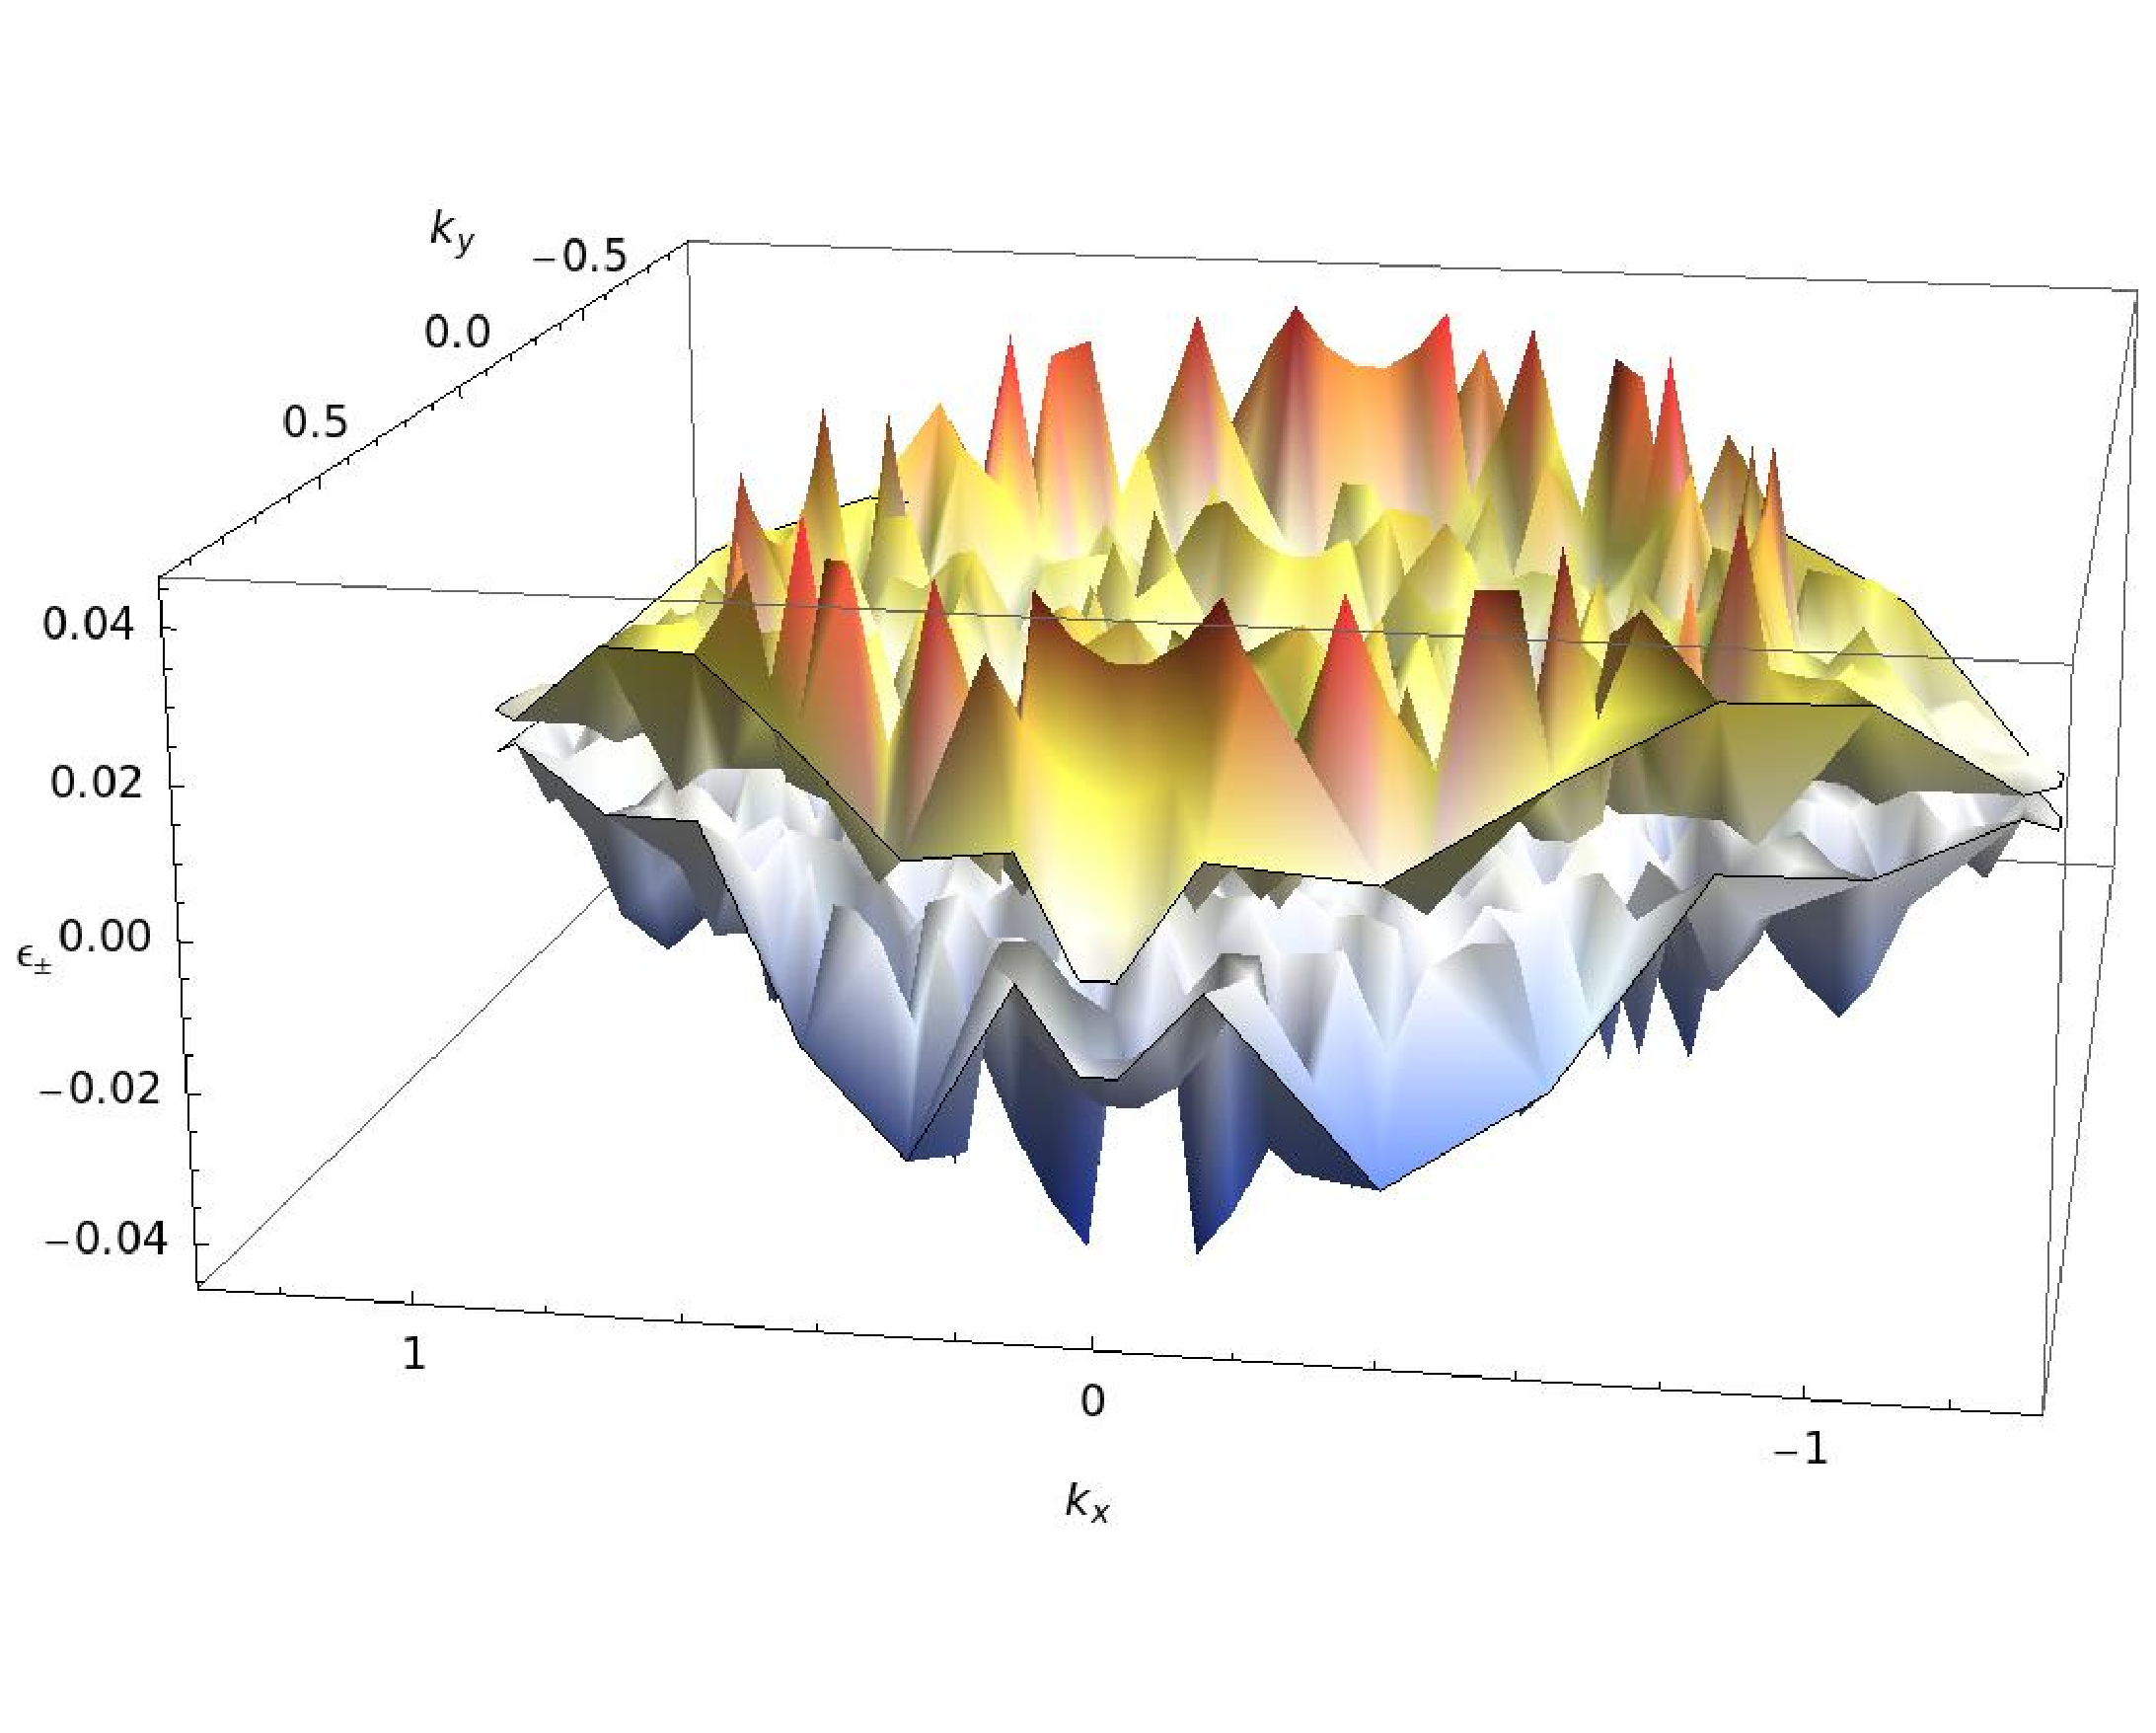
\epsfig{file=bands_3d.eps,height=4.5in,width=6.5in}
\caption{(Color online) Band structure for anisotropic graphene for parameters in table~\ref{tab:params:tau}. Shown here are plots of $\epsilon^\pm_{\bf k}$ as a function of crystal momentum ${\bf k}$ for the 2d honeycomb lattice in fig~\ref{fig:potn} within the FBZ bound by the lines in eqns~\ref{eq:bzone}.}
\label{fig:bands:3d}
\end{figure}
\begin{figure}[h!bt]
\ 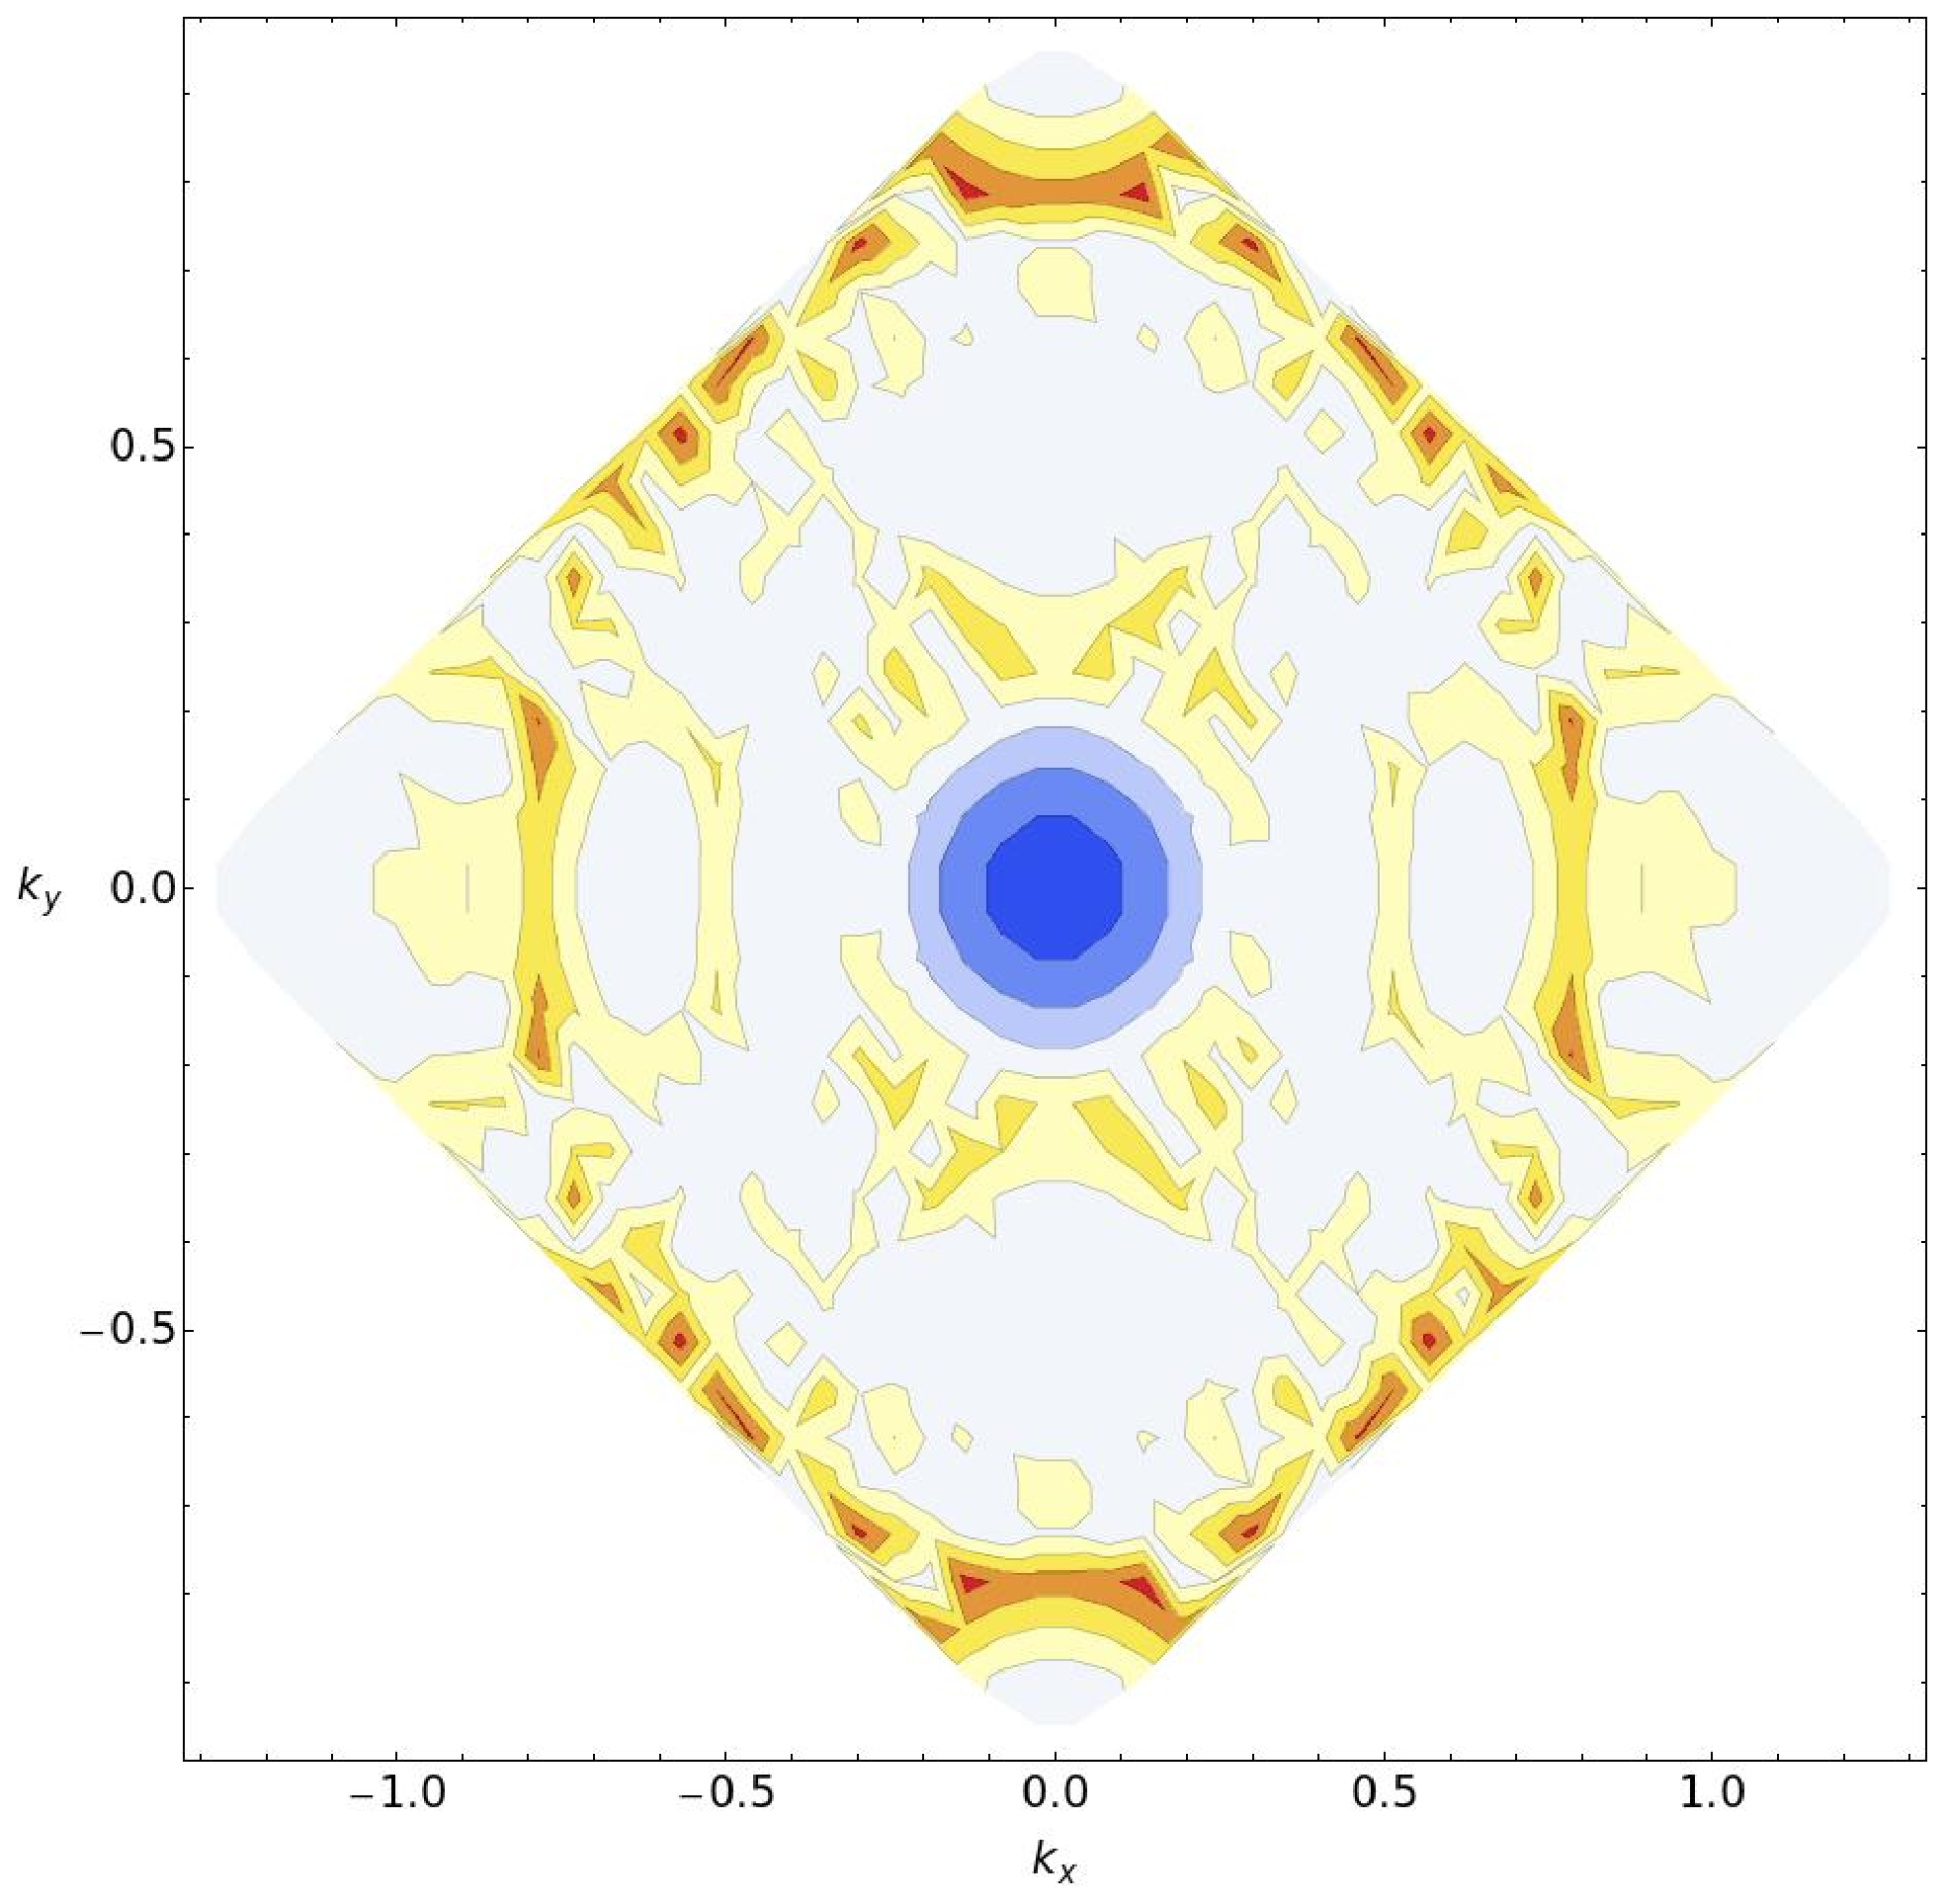
\epsfig{file=lower_band_contour.eps,height=4.5in,width=4.5in}
\caption{(Color online) Band structure for anisotropic graphene for parameters in table~\ref{tab:params:tau}. Shown here are 2d contour plots of $\epsilon^-_{\bf k}$ as a function of crystal momentum ${\bf k}$ for the 2d honeycomb lattice in fig~\ref{fig:potn} within the FBZ bound by the lines in eqns~\ref{eq:bzone}. Also see the full band structure in fig~\ref{fig:bands:3d}.}
\label{fig:lband:contour}
\end{figure}
\begin{thebibliography}{99}
\bibitem{laetitia}
L. Tarruell, D. Greif, T. Uehlinger, G. Jotzu and T. Esslinger, arXiv:1111.5020 (2011)
\bibitem{lee:bandstructure}
K. Lee, B. Gremaud, R. Han, B. Englert, and C. Miniatura, Phys. Rev. A {\bf 80}, 043411 (2009)
\bibitem{rossler}
Ulrich R\"o\ss ler, \textit{Solid State Theory: An Introduction},Springer; 2nd ed. edition (September 10, 2009).
\end{thebibliography}
\end{document}


